
Se hizo inicialmente un cálculo rápido de los valores necesarios para los resistores para lograr el punto Q requerido, luego se refinaron por simulación estos valores, para finalmente llevar a valores comerciales de la serie \textbf{E24} (5 \%) o \textbf{E96} (1 \%), figura~\figref{fig:fig_q_point}. Se utilizaron los de la serie al 1 \% para aquellos resistores que deben estar apareados (espejo de corriente) y para aquellos resistores que fijan la polarización o forman parte de la red de realimentación, en este último caso, también deberían utilizarse resistores de film de óxido metálico, por ser los resistores con mayor estabilidad térmica. En el cuadro~\tableref{table:table_resistors} se muestran los resistores seleccionados y su tipo, y en el cuadro~\tableref{table:table_qpoint} se resumen los valores de polarización finalmente obtenidos. \\

El capacitor $C_{1}$ que se coloca para impedir que continua aplicada al circuito por la fuente de la señal de audio, o una etapa previa, altere la polarización, debería ser un capacitor electrolítico no polarizado, y su valor de $100 \si[per-mode=symbol]{\micro\farad}$ se seleccionó para cumplir con una frecuencia de corte inferior de como máximo $20 \si[per-mode=symbol]{\hertz}$, y no influir significativamente en el THD a bajas frecuencias. Con un valor de $47 \si[per-mode=symbol]{\micro\farad}$ sería suficiente para cumplir con la frecuencia de corte inferior, pero su influencia sobre el THD se hace apreciable incluso a $1 \si[per-mode=symbol]{\kilo\hertz}$ \\

El capacitor $C_{2}$ de $1000 \si[per-mode=symbol]{\micro\farad}$ se seleccionó para que no tenga efecto apreciable sobre el THD, especialmente a bajas frecuencias, y debería ser un capacitor electrolítico de buena calidad, de bajo ESR y no polarizado. La calidad de este capacitor es crítica por hallarse en la red de realimentación, influyendo directamente en la calidad y estabilidad del amplificador. En un circuito mas completo deberían agregarse diodos que protejan este capacitor de un valor de tensión que podría aparecer a la salida, que supere su máxima tensión de trabajo. \\

El capacitor $C_{C}$, de $39 \si[per-mode=symbol]{\pico\farad}$, que se coloca para realizar la compensación de Miller, debería ser un capacitor de poliestireno o poliéster.


\clearpage

\begin{figure}[H] %htb
\begin{center}
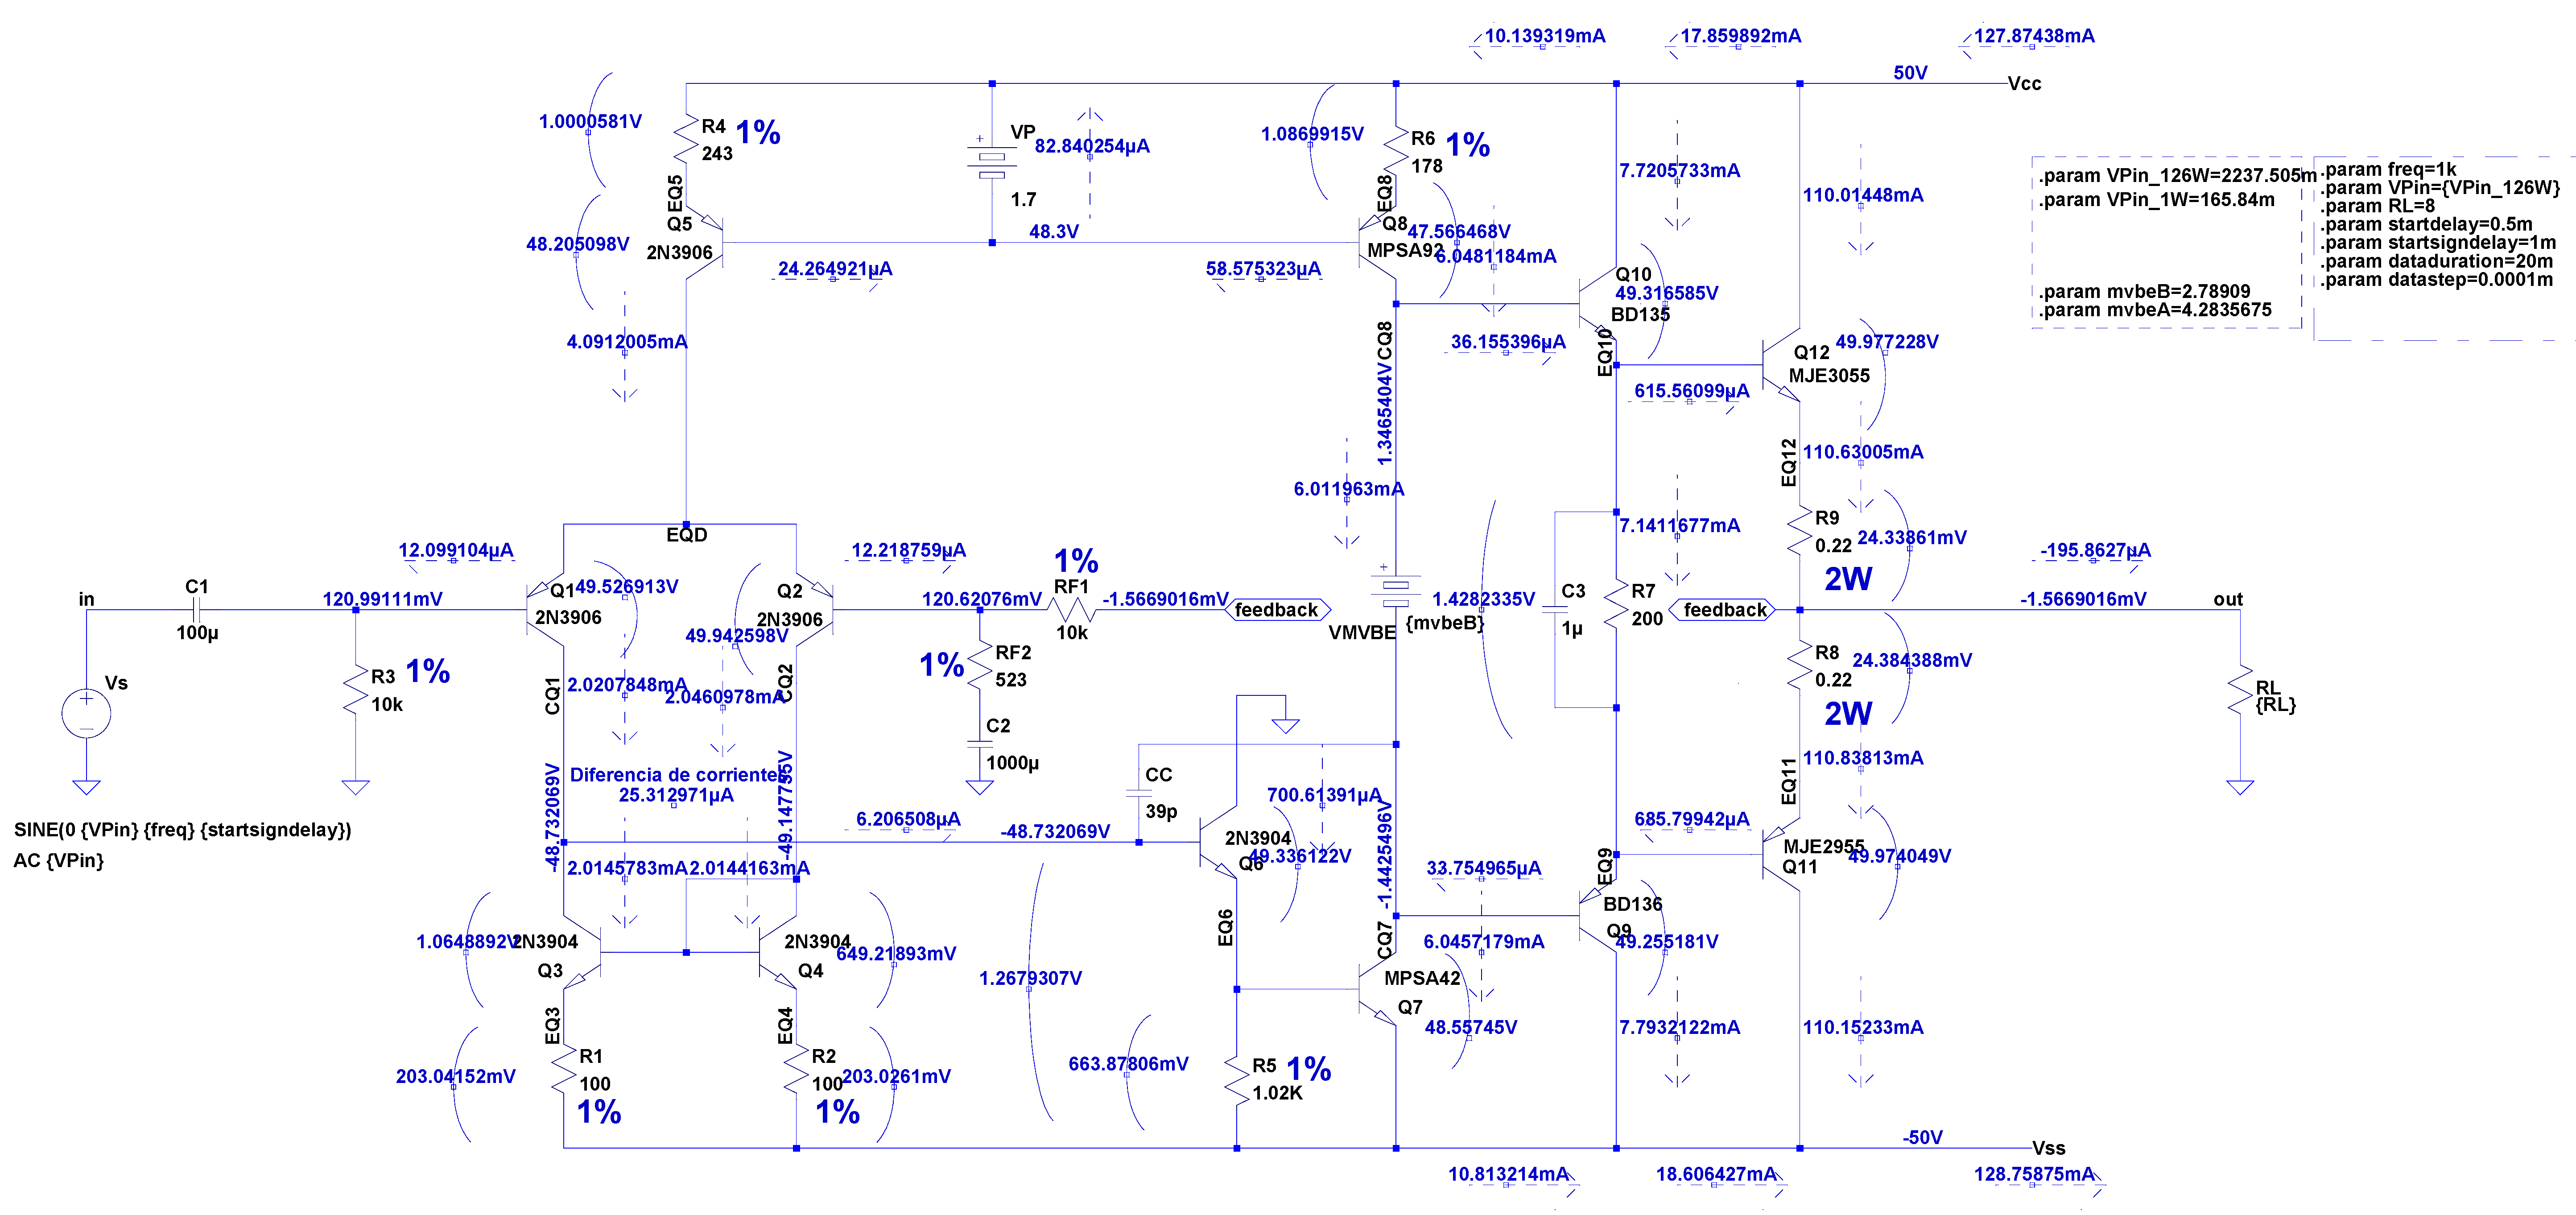
\includegraphics[width=0.93 \textheight, angle=90]{./img/qpoint/amplifier_qpoint.png}
\caption{\label{fig:fig_q_point}\footnotesize{Punto de reposo.}}
\end{center}
\end{figure}

\clearpage



%% \noindent
%% \begin{center}
 
%%\begin{spacing}{1}  
\begin{table}[H]  %%\centering

    \setlength\arrayrulewidth{1.5pt}
    \arrayrulecolor{white}
    \def\clinecolor{\hhline{|>{\arrayrulecolor{white}}-%
    >{\arrayrulecolor{white}}|-|-|-|-|-|-|-|-|-|-|-|-|}}
\resizebox{0.7 \textwidth}{!}{% 
       
\begin{tabularx}{1 \textwidth}%
    {|
    >{\columncolor{white} \centering\arraybackslash}m{0.15\textwidth}
     |
    >{\columncolor{white} \centering\arraybackslash}m{0.09\textwidth}
     |
    >{\columncolor{white} \centering\arraybackslash}m{0.09\textwidth}
     |
    >{\columncolor{white} \centering\arraybackslash}m{0.09\textwidth}
     |
    >{\columncolor{white} \centering\arraybackslash}m{0.09\textwidth}
     |
    >{\columncolor{white} \centering\arraybackslash}m{0.09\textwidth} 
     |
    >{\columncolor{white} \centering\arraybackslash}m{0.09\textwidth}  
     |
    >{\columncolor{white} \centering\arraybackslash}m{0.09\textwidth}  
     |
    >{\columncolor{white} \centering\arraybackslash}m{0.09\textwidth} 
     |
    >{\columncolor{white} \centering\arraybackslash}m{0.09\textwidth}  
     |
    >{\columncolor{white} \centering\arraybackslash}m{0.09\textwidth} 
     |
    >{\columncolor{white} \centering\arraybackslash}m{0.09\textwidth} 
     |
    }
    \rowcolor{HeadersColor} \cellcolor{white} \thead{}  & \thead{R1} & \thead{R2} & \thead{R3} & \thead{R4} & \thead{R5} & \thead{R6} & \thead{R7} & \thead{R8} & \thead{R9} & \thead{RF1} & \thead{RF2} \\  
    \hhline{|-|-|-|-|-|-|-|-|-|-|-|-|}
    \rowcolor{Butter!20} \cellcolor{Butter!40} $R$ [$\si[per-mode=symbol]{\ohm}$] & \num{100} & \num{100} & \num{10e3} & \num{243} & \num{1.02e3} & \num{178} & \num{200} &  \num{.22} & \num{0.22} & \num{10e3} & \num{523}  \\
    \hhline{|-|-|-|-|-|-|-|-|-|-|-|-|}
    \rowcolor{gray!20} \cellcolor{gray!40} $Tolerancia$ [$\si[per-mode=symbol]{\percent}$] & \num{1} & \num{1} & \num{1} & \num{1} & \num{1} & \num{1} & \num{5} &  \num{5} & \num{5} & \num{1} & \num{1} \\
    \hhline{|-|-|-|-|-|-|-|-|-|-|-|-|}
    \rowcolor{gray!20} \cellcolor{gray!40} $Potencia$ [$\si[per-mode=symbol]{\watt}$] & $\frac{1}{8}$ & $\frac{1}{8}$ & $\frac{1}{8}$ & $\frac{1}{8}$ & $\frac{1}{8}$ & $\frac{1}{8}$ & $\frac{1}{8}$ &  \num{2} & \num{2} & $\frac{1}{8}$ & $\frac{1}{8}$ \\
    \hhline{|-|-|-|-|-|-|-|-|-|-|-|-|}    
    \rowcolor{gray!20} \cellcolor{gray!40} TIPO & Metal Film & Metal Film & Metal Film & Metal Film & Metal Film & Metal Film & Carbon Film & Wired & Wired & Metal Oxide Film & Metal Oxide Film \\
    \end{tabularx}}
	\caption{\footnotesize{Resistores seleccionados.}}
	\label{table:table_resistors}
\end{table}
%%\end{spacing}

%% \end{center}




%% \noindent
%% \begin{center}
 
%%\begin{spacing}{1}  
\begin{table}[H]  %%\centering

    \setlength\arrayrulewidth{1.5pt}
    \arrayrulecolor{white}
    \def\clinecolor{\hhline{|>{\arrayrulecolor{white}}-%
    >{\arrayrulecolor{white}}|-|-|-|-|-|-|-|-|-|-|-|-|-|}}
\resizebox{0.66 \textwidth}{!}{% 
       
\begin{tabularx}{1 \textwidth}%
    {|
    >{\columncolor{white} \centering\arraybackslash}m{0.13\textwidth}
     |
    >{\columncolor{white} \centering\arraybackslash}m{0.09\textwidth}
     |
    >{\columncolor{white} \centering\arraybackslash}m{0.09\textwidth}
     |
    >{\columncolor{white} \centering\arraybackslash}m{0.09\textwidth}
     |
    >{\columncolor{white} \centering\arraybackslash}m{0.09\textwidth}
     |
    >{\columncolor{white} \centering\arraybackslash}m{0.09\textwidth} 
     |
    >{\columncolor{white} \centering\arraybackslash}m{0.09\textwidth}  
     |
    >{\columncolor{white} \centering\arraybackslash}m{0.09\textwidth}  
     |
    >{\columncolor{white} \centering\arraybackslash}m{0.09\textwidth} 
     |
    >{\columncolor{white} \centering\arraybackslash}m{0.09\textwidth}  
     |
    >{\columncolor{white} \centering\arraybackslash}m{0.09\textwidth} 
     |
    >{\columncolor{white} \centering\arraybackslash}m{0.09\textwidth} 
     |
    >{\columncolor{white} \centering\arraybackslash}m{0.09\textwidth} 
     |
    }
    \rowcolor{HeadersColor} \cellcolor{white} \thead{}  & \thead{Q1} & \thead{Q2} & \thead{Q3} & \thead{Q4} & \thead{Q5} & \thead{Q6} & \thead{Q7} & \thead{Q8} & \thead{Q9} & \thead{Q10} & \thead{Q11} & \thead{Q12} \\
    
    \hhline{|-|-|-|-|-|-|-|-|-|-|-|-|-|}
    \rowcolor{gray!20} \cellcolor{gray!40} MODEL & 2N3906 & 2N3906 & 2N3904 & 2N3904 & 2N3906 & 2N3904 & MPSA42 & MPSA92 & BD136 & BD135 & MJE2955 & MJE3055  \\
    \hhline{|-|-|-|-|-|-|-|-|-|-|-|-|-|}
    \rowcolor{Butter!20} \cellcolor{Butter!40} $I_{C}$ [$\si[per-mode=symbol]{\ampere}$] & \num{2.02e-3} & \num{2.05e-3} & \num{2.01e-3} & \num{2.01e-3} & \num{4.09e-3} & \num{700.61e-6} & \num{6.05e-3} &  \num{6.05e-3} & \num{7.79e-3} & \num{7.72e-3} & \num{110.00e-3} & \num{110.14e-3}  \\
    \hhline{|-|-|-|-|-|-|-|-|-|-|-|-|-|}
    \rowcolor{gray!20} \cellcolor{gray!40} $gm$ [$\si[per-mode=symbol]{\milli\ampere\per\volt}$] & \num{56.00} & \num{56.60} & \num{48.10} & \num{48.10} & \num{111.00} & \num{17.50} & \num{20.40} & \num{22.90} & \num{300} & \num{298.00} & \num{4060.00}  & \num{4170.00} \\
    \hhline{|-|-|-|-|-|-|-|-|-|-|-|-|-|}
    \rowcolor{gray!20} \cellcolor{gray!40} $r_{o}$ [$\si[per-mode=symbol]{\ohm}$] & \num{92.7e+03} & \num{91.7e+03} & \num{462.0e+03} & \num{462.0e+03} & \num{45.3e+03} & \num{1.41e+06} & \num{24.5e+03} & \num{24.3e+03} & \num{18.5e+03} & \num{21.3e+03} & \num{1.36e+03} & \num{903.0}  \\
    \hhline{|-|-|-|-|-|-|-|-|-|-|-|-|-|}
    \rowcolor{gray!20} \cellcolor{gray!40} $\beta [AC]$ & 174 & 174 & 140 & 140 & 170 & 143 & 157 & 108 & 242  & 223 & 162 & 196  \\
    \hhline{|-|-|-|-|-|-|-|-|-|-|-|-|-|}
    \rowcolor{gray!20} \cellcolor{gray!40}  $r_{\pi}$ [$\si[per-mode=symbol]{\ohm}$] & \num{3.10e3} & \num{3.07e3} & \num{2.90e3} & \num{2.90e3} & \num{1.53e3}  & \num{8.17e3}  & \num{772.0} & \num{472.0} & \num{806.0} & \num{748.0} & \num{40.0} & \num{47.0}  \\
    \hhline{|-|-|-|-|-|-|-|-|-|-|-|-|-|}
    \rowcolor{gray!20} \cellcolor{gray!40} $f_{T}$ [$\si[per-mode=symbol]{\mega\hertz}$] & \num{210.00} & \num{211.00} & \num{227.00} & \num{222.00} & \num{247.00} & \num{164.00} & \num{74.90} & \num{81.10} & \num{115.00} & \num{178.00} & \num{6.80} & \num{4.24}  \\         
    \end{tabularx}}
	\caption{\footnotesize{$I_{C_{Q}}$ y elementos del modelo de pequeña señal de los transistores.}}
	\label{table:table_qpoint}
\end{table}
%%\end{spacing}

%% \end{center}




